%! suppress = MissingLabel
%! suppress = LineBreak

% CLI args https://tex.stackexchange.com/a/1501
\newif\ifhandout
\input{flags}

%! suppress = MissingLabel
%! suppress = DocumentclassNotInRoot
%! suppress = DiscouragedUseOfDef

% * Make friends tikz & colors
%   https://en.wikibooks.org/wiki/LaTeX/Colors
% * To enable vertical top alignment globally
%   https://tex.stackexchange.com/questions/9889/positioning-content-at-the-top-of-a-beamer-slide-by-default
% * Set handout from CLI
%   https://tex.stackexchange.com/a/1501
\ifhandout
\documentclass[usenames, dvipsnames, handout]{beamer} % https://tex.stackexchange.com/questions/224091/beamer-how-to-disable-pause-temporarily
\else
\documentclass[usenames, dvipsnames]{beamer}
\fi
% ------------------------------------------------

% Graphics
\usepackage{color}
\usepackage{tabularx}
\usepackage{tikz}
% https://tikz.dev/tikz-graphs
\usetikzlibrary{positioning, shapes.geometric, arrows, automata, graphs}
\tikzset{
    expr/.style={ellipse, draw=gray!60, fill=gray!5, very thick, minimum size=7mm, yshift=0.7cm},
    hexpr/.style={ellipse, draw=gray!60, fill=blue!15, very thick, minimum size=7mm, yshift=0.7cm},
    stmt/.style={rectangle, draw=gray!60, fill=gray!5, very thick, minimum size=5mm, yshift=0.7cm},
    decl/.style={rectangle, draw=blue!60, fill=gray!5, very thick, minimum size=5mm, yshift=0.7cm},
    hdecl/.style={rectangle, draw=blue!60, fill=blue!15, very thick, minimum size=5mm, yshift=0.7cm},
    subtree/.style={shape border rotate=90, isosceles triangle, draw=gray!60, fill=gray!5, very thick, minimum size=5mm, yshift=0.0cm},
}
\usepackage{blkarray}
\usepackage{graphicx}
\usepackage{forest} % https://tex.stackexchange.com/questions/198405/how-to-change-the-color-of-subtrees-in-tikz-qtree
% ------------------------------------------------

% Math
\usepackage{amsmath, amsfonts}
\usepackage{amssymb}
\usepackage{proof}
\usepackage{mathrsfs}
% Crossed-out symbols
% https://tex.stackexchange.com/questions/75525/how-to-write-crossed-out-math-in-latex
\usepackage[makeroom]{cancel}
\usepackage{mathtools}
% ------------------------------------------------

% Additional font sizes
% https://www.overleaf.com/learn/latex/Questions/How_do_I_adjust_the_font_size%3F
\usepackage{moresize}
% Additional colors
% https://www.overleaf.com/learn/latex/Using_colours_in_LaTeX
\usepackage{xcolor}
% Textual math symbols
\usepackage{textcomp}
% ------------------------------------------------

% Language
\usepackage[utf8] {inputenc}
\usepackage[T2A] {fontenc}
\usepackage[english, russian] {babel}
\usepackage{indentfirst, verbatim}
\usetikzlibrary{cd, babel}
% ------------------------------------------------

% Fonts: https://sites.math.washington.edu/~reu/docs/latex_symbols.pdf
\usepackage{stmaryrd}
\usepackage{cmbright}
\usepackage{wasysym}
\usepackage[weather]{ifsym} % https://tex.stackexchange.com/questions/100424/how-to-use-the-ifsym-package
% https://tex.stackexchange.com/questions/615300/pdflatex-builtin-glyph-names-is-empty
\pdfmapline{=dictsym DictSym <dictsym.pfb}
\pdfmapline{=pigpen <pigpen.pfa}
\usepackage{dictsym}
% ------------------------------------------------

% Code
% * Needs -shell-escape build flag
%   https://tex.stackexchange.com/questions/99475/how-to-invoke-latex-with-the-shell-escape-flag-in-texstudio-former-texmakerx
% * Set build directory
%   https://tex.stackexchange.com/questions/339931/latex-minted-package-using-custom-output-directory-build
\usepackage{minted}
\setminted{xleftmargin=\parindent, autogobble, escapeinside=\#\#}
% ------------------------------------------------

% Template
\usetheme{CambridgeUS}
\usecolortheme{dolphin}
% https://tex.stackexchange.com/questions/231439/beamer-how-to-make-font-larger-for-page-numbers
\setbeamerfont{headline}{size=\scriptsize}
\setbeamerfont{footline}{size=\scriptsize}
% Remove heddline
% https://tex.stackexchange.com/questions/33146/how-could-i-remove-a-header-in-a-beamer-presentation
%\setbeamertemplate{headline}{}
% Slide sizes
% https://tex.stackexchange.com/questions/56768/how-to-set-a-small-default-font-size-with-beamer
%\geometry{paperwidth=140mm,paperheight=105mm} % 4:3
\geometry{paperwidth=168mm,paperheight=105mm} % 16:10
% Remove navigation bar
% https://stackoverflow.com/questions/3210205/how-to-get-rid-of-navigation-bars-in-beamer
\beamertemplatenavigationsymbolsempty
% ------------------------------------------------

% Bullets
% https://9to5science.com/change-bullet-style-formatting-in-beamer
% https://tex.stackexchange.com/questions/185742/i-need-to-change-color-of-beamer-itemize-and-subitem-separately
\setbeamertemplate{itemize item}{\scriptsize\raise1.25pt\hbox{\donotcoloroutermaths$\blacktriangleright$}}
\setbeamertemplate{itemize subitem}{\scriptsize\raise1.5pt\hbox{\donotcoloroutermaths$\blacktriangleright$}}
\setbeamertemplate{itemize subsubitem}{\tiny\raise1.5pt\hbox{\donotcoloroutermaths$\blacktriangleright$}}
\setbeamertemplate{enumerate item}{\insertenumlabel.}
\setbeamertemplate{enumerate subitem}{\insertenumlabel.\insertsubenumlabel}
\setbeamertemplate{enumerate subsubitem}{\insertenumlabel.\insertsubenumlabel.\insertsubsubenumlabel}
% ------------------------------------------------

% Table of contents format
% https://tex.stackexchange.com/questions/642927/format-table-of-contents-in-beamer
\setbeamertemplate{section in toc}{%
        {\color{blue}\inserttocsectionnumber.}
    \inserttocsection\par%
}
\setbeamertemplate{subsection in toc}{%
        {\color{blue}\hspace{1em}\scriptsize\raise1.25pt\hbox{\donotcoloroutermaths$\blacktriangleright$}}
    \inserttocsubsection\par%
}
\setbeamertemplate{subsubsection in toc}{%
        {\color{blue}\hspace{2em}\tiny\raise1.25pt\hbox{\donotcoloroutermaths$\blacktriangleright$}}
    \inserttocsubsubsection\par%
}
% ------------------------------------------------

% Misc
\usepackage{multicol}
\usepackage{hyperref}
\usepackage{soul} % https://tex.stackexchange.com/questions/23711/strikethrough-text
% ------------------------------------------------

% Fix \pause for amsmath package envs (black black magic)
% https://tex.stackexchange.com/questions/16186/equation-numbering-problems-in-amsmath-environments-with-pause/75550#75550
% https://tex.stackexchange.com/questions/6348/problem-with-beamers-pause-in-alignments
%! suppress = Makeatletter
\makeatletter
\let\save@measuring@true\measuring@true
\def\measuring@true{%
    \save@measuring@true
    \def\beamer@sortzero##1{\beamer@ifnextcharospec{\beamer@sortzeroread{##1}}{}}%
    \def\beamer@sortzeroread##1<##2>{}%
    \def\beamer@finalnospec{}%
}
%! suppress = Makeatletter
\makeatother
% ------------------------------------------------

% Sections
\newcommand{\sectionplan}[1]{\section{#1}%
    \begin{frame}[noframenumbering]{Содержание}
        \tableofcontents[currentsection]
    \end{frame}
}
\newcommand{\subsectionplan}[1]{\subsection{#1}%
    \begin{frame}[noframenumbering]{Содержание}
        \tableofcontents[currentsubsection]
    \end{frame}
}
% ------------------------------------------------

% Footnotes
\renewcommand{\thefootnote}{\arabic{footnote}}
\renewcommand{\thempfootnote}{\arabic{mpfootnote}}
% https://tex.stackexchange.com/questions/28465/multiple-footnotes-at-one-point
\usepackage{fnpct}
% ------------------------------------------------

% Links
% Colors also links on slide foot.
%\hypersetup{
%    colorlinks=true,
%    citecolor=blue,
%    linkcolor=blue,
%    urlcolor=blue
%}
% ------------------------------------------------

% Appendix
% Slide numbers
% https://tex.stackexchange.com/questions/70448/dont-count-backup-slides
\usepackage{appendixnumberbeamer}
\newcommand{\backupbegin}{
    \newcounter{framenumbervorappendix}
    \setcounter{framenumbervorappendix}{\value{framenumber}}
}
\newcommand{\backupend}{
    \addtocounter{framenumbervorappendix}{-\value{framenumber}}
    \addtocounter{framenumber}{\value{framenumbervorappendix}}
}
% ------------------------------------------------

% Custom commands
% * Decor
\newcommand{\newtopic}[0]{$+$} % item: new topic on "in previous series"
\newcommand{\then}{$\Rightarrow$} % item: consequences
\newcommand{\pop}[0]{\SunCloud} %item:  general eduation
\newcommand{\popslide}[0]{(\pop)}
\newcommand{\advanced}[0]{$\varhexstar$} % item: advanced science
\newcommand{\advancedslide}[0]{(\advanced)}
\newcommand{\practical}[0]{\dstechnical} % item: practical programming notions
\newcommand{\practicalslide}[0]{(\practical)}
\newcommand{\todo}[0]{todo} % item: question
\newcommand{\answer}[0]{\Lightning} % item: answer to the previous question
\newcommand{\eg}[0]{e.g.} % item: example
\newcommand{\defi}[0]{$\Delta$} % item: definition on smth
\newcommand{\textdefi}[1]{\textbf{#1}}
\newcommand{\positive}{$+$} % item: pros
\newcommand{\negative}{{\color{red} $-$}} % item: cons
\newcommand%! suppress = EscapeHashOutsideCommand
\NB[1][0.3]{N\kern-#1em{B}} % default kern amount: -0.3em
\renewcommand{\emph}[1]{{\color{blue} \textit{#1}}}
\newcommand{\vocab}[1]{\textbf{#1}} % item: important new word
% * Lambda calculi
\newcommand{\comb}[1]{\mathbf{#1}} % defined combinator
\newcommand{\term}[1]{\mathbf{#1}} % predefined lambda-term reference
\newcommand{\termdef}{\coloneqq} % lamda term binding
\newcommand{\step}{\rightsquigarrow} % reduction step
\newcommand{\sstep}{\twoheadrightarrow} % multiple steps reduction
\newcommand{\ap}{~} % lambda-term application
\newcommand{\subst}[3]{\left[#2 \mapsto #3 \right] #1} % substitution
\newcommand{\eqbeta}{=_\beta} % beta equality
\newcommand{\eqeta}{=_\eta} % eta-equality
\newcommand{\eqt}{=} % tree-equality of terms
\newcommand{\tlist}[1]{\term{[}#1\term{]}} % list-term
% * Legacy
%\newcommand{\err}[0]{\textcolor{red}{ошибка}} % compilation error

% ------------------------------------------------

% Speaker notes
% https://tex.stackexchange.com/questions/114219/add-notes-to-latex-beamer
% https://tex.stackexchange.com/questions/35444/split-beamer-notes-across-multiple-notes-pages/35496#35496
%\setbeameroption{show notes on second screen=right} % enable speaker notes
%--------------------------------------

\author[]{Андрей Стоян, Илья Колегов, Дмитрий Халанский}
\institute[MSE ITMO]{MSE ITMO}


\title[2. Рекурсия в $\lambda$-исчислении]{Практика 2. Рекурсия в $\lambda$-исчислении}
\date{осень 2024}

\begin{document}

    \setcounter{framenumber}{-1}
    \maketitle

    \begin{frame}{В предыдущих сериях}
        \begin{itemize}
            \item Синтаксис и семантика $\lambda$-исчисления
            \item Абстракция по данным в $\lambda$-исчислении: кортежи, натуральные числа, логические величины
            \item[\newtopic] Нормальные формы
            \item[\newtopic] Рекурсия и $\comb{Y}$-комбинатор
            \item[\newtopic] Стратегии редукции
        \end{itemize}
    \end{frame}

    \begin{frame}[noframenumbering]{Содержание}
        \tableofcontents
    \end{frame}


    \sectionplan{Примитивная рекурсия}

    \begin{frame}[fragile]{Цикл по заданному интервалу}
        \begin{minted}{Python}
            def rec(f, ini, n):
                acc = ini
                for i in range(0, n):
                    acc = f(i, acc)
                return acc
        \end{minted}
        \begin{itemize}
            \item[\todo] Перепишите рекурсивно
            \item[\answer] \pause
        \end{itemize}
        \begin{minted}{Python}
            def rec(f, ini, n): #\pause#
                if n == 0: #\pause#
                    return ini
                else: #\pause#
                    return f(n - 1, rec(f, ini, n - 1))
        \end{minted}
    \end{frame}

    \begin{frame}[fragile]{Идея трансляции в $\lambda$-исчисление}
        \begin{itemize}
            \item Пример вычисления:
            \begin{minted}[escapeinside=??]{python}
                      rec(f, ini, 3)
                ?$\step_\beta$??\pause? f(2,   rec(f, ini, 2))
                ?$\step_\beta$??\pause? f(2, f(1,   rec(f, ini, 1)))
                ?$\step_\beta$??\pause? f(2, f(1, f(0, rec(f, ini, 0))))
                ?$\step_\beta$??\pause? ?\framebox{f(2, f(1, f(0, ini)))}?
            \end{minted}
            \item[\todo] Какая будет идея трансляции?
            \item[\answer] \pause Похоже на числа Чёрча
            \item[\answer] Последовательно преобразуется пара из индекса и предыдущего результата
        \end{itemize}
    \end{frame}

    \begin{frame}[fragile]{Примитивная рекурсия в $\lambda$-исчислении}
        \begin{columns}[onlytextwidth]
            \begin{column}{0.385\textwidth}
                \vspace{-1em}
                \begin{minted}{Python}
                    def rec(f, ini, n):
                        if n == 0:
                            return ini
                        else:
                            res = rec(f, ini, n - 1)
                            return f(n - 1, res)
                \end{minted}
                \vspace{0.5em}
                Вычисляется в
                \begin{minted}{python}
                    f(2, f(1, f(0, ini)))
                \end{minted}
                \vspace{0.5em}
                Нужно выразить в виде
                $s \ap (s \ap (s \ap z))$.
            \end{column}\hfill%
            \pause
            \begin{column}{0.585\textwidth}
                \begin{itemize}
                    \item Из итерации в итерацию передаём пару из номера итерации и результата предыдущей
                    \item Начальное состояние --- $\term{start} \ap ini \termdef \pause \term{pair} \ap \term{0} \ap ini$
                    \item Одна итерация:
                    \[
                        \term{step} \pause \ap f \ap (\term{pair} \ap i \ap res)
                        \termdef
                        \term{pair} \ap (\term{suc} \ap i) \ap (f \ap i \ap res)
                    \] \vspace{-1em}
                    \item Итерирование
                    \[
                        \term{iter} \ap f \ap ini \ap n
                        \termdef
                        \pause \term{natElim} \ap n \ap (\term{step} \ap f) \ap (\term{start} \ap ini)
                    \] \vspace{-1em}
                    \item И наконец
                    \[
                        \term{rec} \ap f \ap ini \ap n
                        \termdef
                        \pause \term{snd} \ap (\term{iter} \ap f \ap ini \ap n)
                    \] \vspace{-1em}
                \end{itemize}
            \end{column}
        \end{columns}
    \end{frame}

    \begin{frame}[fragile]{Примеры применения примитивной рекурсии}
        \begin{block}{Свойство примитивной рекурсии}
            \vspace{-0.5em}

            \[\term{rec}~f~ini~n \eqbeta \pause f~(n-1)~(f~(n-2)~(\cdots~(f~1~(f~0~ini))\cdots))\]

            \vspace{-1.5em}
        \end{block}
        \vspace{1em}
        \begin{itemize}
            \item[\todo] Реализуйте функцию суммирования чисел от $1$ до $n$
            \item[\todo] Реализуйте факториал
            \item[\todo] Реализуйте $\term{pred}$
            \item[\answer] \pause $\term{sum} \ap n \termdef \term{rec} \ap (\lambda i \ap res \ldotp \term{plus} \ap (\term{suc} \ap i) \ap res) \ap \term{0} \ap n$
            \item[\answer] \pause $\term{fac} \ap n
            \termdef
            \term{rec}
            \ap (\lambda \pause i \ap res \ldotp \term{mult} \ap (\term{suc} \ap i) \ap res)
            \ap \term{1} \ap n$
            \item[\answer] $\term{pred} \ap n \termdef \pause \term{rec}~\term{K}~\term{0} \ap n$
            \item Во всех случаях можно сделать $\eta$-редукцию
        \end{itemize}
    \end{frame}

    \begin{frame}[fragile]{Проверка факториала}
        \pause
        \begin{itemize}
            \item $
            \term{fac}~\term{2} \step_{\beta}
            \term{snd}~(\term{2}~(\term{step}~(\lambda i~r\ldotp \term{mult}~(\term{suc}~i)~r))~(\term{pair}~\term{0}~\term{1})) \step_{\beta}
            \term{snd}~(\term{step}~(\lambda i~r\ldotp \term{mult}~(\term{suc}~i)~r)~((\term{step}~(\lambda i~r\ldotp \term{mult}~(\term{suc}~i)~r))~(\term{pair}~\term{0}~\term{1}))) \step_{\beta}
            \term{snd}~(\term{step}~(\lambda i~r\ldotp \term{mult}~(\term{suc}~i)~r)~(\term{pair}~(\term{suc}~\term{0})~((\lambda i~r\ldotp \term{mult}~(\term{suc}~i)~r)~\term{0}~\term{1}))) \step_{\beta}
            \term{snd}~(\term{step}~(\lambda i~r\ldotp \term{mult}~(\term{suc}~i)~r)~(\term{pair}~\term{1}~(\term{mult}~(\term{suc}~\term{0})~\term{1}))) \step_{\beta}
            \term{snd}~(\term{step}~(\lambda i~r\ldotp \term{mult}~(\term{suc}~i)~r)~(\term{pair}~\term{1}~\term{1})) \step_{\beta}
            \term{snd}~(\term{pair}~(\term{suc}~\term{1})~((\lambda i~r\ldotp \term{mult}~(\term{suc}~i)~r)~\term{1}~\term{1})) \step_{\beta}
            (\lambda i~r\ldotp \term{mult}~(\term{suc}~i)~r)~\term{1}~\term{1} \step_{\beta}
            \term{mult}~(\term{suc}~\term{1})~\term{1} \step_{\beta}
            \term{2}
            $
            \item \pause Да ну серьёзно??
            \item \pause Через свойство примитивной рекурсии сильно проще
            \begin{align*}
                \term{fac} \ap \term{3}
                &\step_{\beta} \pause
                f~\term{2}~(
                f~\term{1}~(
                f~\term{0}~\term{1}))
                \\ &\step_{\beta} \pause
                (\lambda i \ap res\ldotp \term{mult}~(\term{suc}~i) \ap res)~\term{2}~(
                f~\term{1}~(
                f~\term{0}~\term{1}))
                \\ &\step_{\beta} \pause
                \term{mult}~(\term{suc}~\term{2})~(
                f~\term{1}~(
                f~\term{0}~\term{1}))
                \\ &\step_{\beta} \pause
                \term{mult}~\term{3}~(
                \term{mult}~\term{2}~(
                \term{mult}~\term{1}~\term{1}))
                \step_{\beta} \pause
                \term{6}
            \end{align*}
            \item Важно грамотно выбирать уровень абстракции
        \end{itemize}
    \end{frame}

    \sectionplan{Комбинатор неподвижной точки}

    \begin{frame}{Рекурсия}
        \begin{itemize}
            \item Одной примитивной рекурсии в языке не достаточно, чтобы быть полным по Тьюрингу
            \item Чтобы добиться полноты, нужна полноценная рекурсия
            \item  В прикладные языки рекурсия встроена --- достаточно в теле именованной функции вызвать её саму
            \item Но у нас в языке нет именованных функций
            \item Договорённость о синонимах не решает проблемы
            \begin{itemize}
                \item Это синтаксическая конвенция, а не семантическая (вычислительная)
                \item $\term{fac} \termdef \cdots \term{fac} \cdots$ --- бесконечное дерево, которое в месте вхождения синонима в правую часть повторяется снова и снова
            \end{itemize}
        \end{itemize}
    \end{frame}

    \begin{frame}{Рекурсивные уравнения на термах}
        Хотим подобрать такой терм $\term{fac}$, чтобы $\term{fac} \ap N \eqbeta \pause \term{if} \ap (\term{iszero} \ap N) \ap \term{1} \ap (\term{mult} \ap N \ap (\term{fac} \ap (\term{pred} \ap N)))$.

        \pause
        \vspace{0.5em}
        Решаем рекурсивное уравнение на термах!
        \begin{enumerate}
            \item \pause Абстрагируемся в левой части по $\term{fac}$ и $N$:
            \[
                \term{fac} \ap N
                \eqbeta
                % https://tex.stackexchange.com/questions/245934/how-can-i-make-underbrace-texts-have-the-normal-text-size
                \underbrace{(\lambda rec \ap n \ldotp \term{if} \ap (\term{iszero} \ap \framebox{n}) \ap \term{1} \ap (\term{mult} \ap \framebox{n} \ap (\framebox{rec} \ap (\term{pred} \ap \framebox{n}))))}_{\textstyle \term{fac'}}
                \ap \term{fac} \ap N
            \]
            \item \pause Делаем в обеих частях $\eta$-редукцию, так как она не портит аппликативного поведения:
            \[
                \term{fac} \eqt_{\beta\eta} \term{fac'} \ap \term{fac}
            \]
            \item \pause То есть $\term{fac}$ --- неподвижная точка отображения $\term{fac'}$!  Найдём её $\comb{Y}$-комбинатором:
            \[
                \term{fac}
                \termdef \pause
                \comb{Y} \ap \term{fac'}
                \eqt_{\beta} \pause
                \comb{Y} \ap (\lambda rec \ap n \ldotp \term{if} \ap (\term{iszero} \ap n) \ap \term{1} \ap (\term{mult} \ap n \ap (rec \ap (\term{pred} \ap n))))
            \]
            \vspace{-1em}
            \item \pause Делаем проверку:
            \begin{align*}
                \term{fac} \ap N
                &\eqbeta \pause
                \comb{Y} \ap \term{fac'} \ap N
                \eqbeta \pause
                \term{fac'} \ap (\comb{Y} \ap \term{fac'}) \ap N
                \\&\eqbeta \pause
                (\lambda rec \ap n \ldotp \term{if} \ap (\term{iszero} \ap \framebox{n}) \ap \term{1} \ap (\term{mult} \ap \framebox{n} \ap (\framebox{rec} \ap (\term{pred} \ap \framebox{n})))) \ap (\comb{Y} \ap \term{fac'}) \ap N
                \\&\eqbeta \pause
                \term{if} \ap (\term{iszero} \ap \framebox{N}) \ap \term{1} \ap (\term{mult} \ap \framebox{N} \ap (\framebox{$\comb{Y} \ap \term{fac'}$} \ap (\term{pred} \ap \framebox{N})))
            \end{align*}
        \end{enumerate}
    \end{frame}

    \begin{frame}{Комбинатор рекурсии (неподвижной точки)}
        \pause
        \vspace{-0.5em}
        \begin{block}{Свойство комбинатора неподвижной точки ($\comb{Y}$ --- пример такого комбинатора)}
            \[
                \underbrace{\comb{Y} \ap F}_{\textstyle X} \eqbeta F \ap (\underbrace{\comb{Y} \ap F}_{\textstyle X})
            \]
        \end{block}
        \[
            \term{fac}
            \termdef
            \comb{Y} \ap \underbrace{(\lambda \framebox{rec} \ap n \ldotp \term{if} \ap (\term{iszero} \ap n) \ap \term{1} \ap (\term{mult} \ap n \ap (\framebox{rec} \ap (\term{pred} \ap n))))}_{\textstyle \term{fac'}}
        \]
        \begin{itemize}
            \item[\todo] Стоп, стоп. Как анонимная функция стала рекурсивной?
            \item[\answer] \pause $\comb{Y}$ передаёт в нашу функцию терм, который ведёт себя ровно так же, как она!\footnote{Получили конечный терм, который в результате вычислений может сколь угодно разрастаться.}
        \end{itemize}
        \pause
        \begin{block}{Договорённость о рекурсивных синонимах}
            Вводим рекурсию как синтаксический сахар для определения выше:
            \vspace{-0.5em}
            \[
                \term{fac} \ap n
                \termdef
                \term{if} \ap (\term{iszero} \ap n) \ap \term{1} \ap (\term{mult} \ap n \ap (\framebox{$\term{fac}$} \ap (\term{pred} \ap n)))
            \]
        \end{block}
    \end{frame}

    \begin{frame}[fragile]{Выбор инструмента: примитивная рекурсия vs рекурсия \practicalslide}
        \begin{itemize}
            \item Примитивная рекурсия
            \begin{itemize}
                \item Задаёт процесс из конечного, заранее заданного, количества шагов
                \item Аналог цикла \mintinline{python}|for in range| в современных языках
            \end{itemize}
            \item Рекурсия
            %! suppress = Ellipsis
            \begin{itemize}
                \item Количество шагов определяется в процессе (и никак иначе: halting problem)
                \item Завершение процесса определяется выполнением произвольного условия (базы рекурсии)
                \item В современных языках выражается рекурсией\footnote{Хвостовая рекурсия полностью эквивалентна обычной, хотя и похожа на примитивную (см. \href{https://en.wikipedia.org/wiki/Trampoline\_(computing)\#High-level_programming}{\color{blue} trampolining}).} и циклом \mintinline{python}|while condition: ...|
            \end{itemize}
            \item Всегда нужно выбирать \emph{наименее могущественный} из подходящих инструментов
            \begin{itemize}
                \item Проще для рассуждений и доказательства свойств
                \item Меньше пространство для ошибок
                \item Скорее всего, код будет эффективнее исполняться
                \item В частности, какие функции примитивно-рекурсивные, а какие --- нет, рассказывает теория вычислимости
            \end{itemize}
        \end{itemize}
    \end{frame}


    \section{Кодирование данных в лямбда-исчислении}

    \subsectionplan{Значения-варианты}

    \begin{frame}[fragile]{\subsecname}
        Одна сущность может быть нескольких различных видов:
        \begin{itemize}
            \item Пользователь может быть авторизованный и не авторизованный
            \item Вершина программы может быть константой, а может --- бинарной операцией
        \end{itemize}
        \pause
        \vspace{1em}
        Хотим, чтобы в зависимости от её вида, сущность обрабатывал разный код:
        \begin{minted}{python}
            def eval(node): #\pause#
                if is_const(node): #\pause#
                    return node.value  # У константы должно быть значение
                elif is_plus(node): #\pause#
                    return eval(node.left) + eval(node.right)  # У плюса - операнды
        \end{minted}
    \end{frame}

    \begin{frame}[fragile]{Моделируем значения-варианты}
        \pause
        \begin{block}{API вариантов}
            \begin{itemize}
                \item Один вариант будем называть ``левым'', второй --- ``правым''
                \item Два конструктора $\term{inl}$ и $\term{inr}$
                \item Элиминатор позволяет выполнить разный код в зависимости от варианта: $\term{either}$
            \end{itemize}
        \end{block}
        \pause
        \begin{block}{Законы вариантов}
            \begin{enumerate}
                \item $\forall f~g~x \pause \ldotp \term{either} \ap f \ap g \ap (\term{inl} \ap x) \eqbeta f \ap x$
                \item $\forall f~g~y \ldotp \term{either} \ap f \ap g \ap (\term{inr} \ap y) \eqbeta g \ap y$
            \end{enumerate}
        \end{block}
        \pause
        \begin{itemize}
            \item[\todo] Что если нужно закодировать больше двух вариантов?
        \end{itemize}
    \end{frame}

    \begin{frame}[fragile]{Тегированное представление вариантов}
        \begin{block}{Законы вариантов}
            \begin{enumerate}
                \item $\forall f~g~x \pause \ldotp \term{either} \ap f \ap g \ap (\term{inl} \ap x) \eqbeta \pause f \ap x$
                \item $\forall f~g~y \ldotp \term{either} \ap f \ap g \ap (\term{inr} \ap y) \eqbeta g \ap y$
            \end{enumerate}
        \end{block}
        \pause
        \begin{block}{Конструкторы}
            \begin{itemize}
                \item Будем приписывать булев тег для различения вариантов
                \item $\term{inl} \ap x \termdef \term{pair} \ap \term{true} \ap x$
                \item $\term{inr} \ap y \termdef \term{pair} \ap \term{false} \ap y$
            \end{itemize}
        \end{block}
        \pause
        \begin{block}{Элиминатор}
            \begin{itemize}
                \item Вызвать нужную функцию в зависимости от тега
                \item $\term{either} \ap f \ap g \ap (\term{pair} \ap tag \ap val) \termdef \term{if} \ap tag \ap (f \ap val) \ap (g \ap val)$
            \end{itemize}
        \end{block}
    \end{frame}

    \begin{frame}[fragile]{Кодирование вариантов ``наоборот''}
        \begin{block}{Законы вариантов}
            \begin{enumerate}
                \item $\forall f~g~x \pause \ldotp \term{either} \ap f \ap g \ap (\term{inl} \ap x) \eqbeta \pause f \ap x$
                \item $\forall f~g~y \ldotp \term{either} \ap f \ap g \ap (\term{inr} \ap y) \eqbeta g \ap y$
            \end{enumerate}
        \end{block}
        \pause
        \begin{block}{Конструкторы}
            \begin{itemize}
                \item Принимают один аргумент
                \item Принимают два действия, из которых выполняют нужное на аргументе
                \item $\term{inl} \ap x \termdef \lambda f~g \ldotp f \ap x$
                \item $\term{inr} \ap y \termdef \lambda f~g \ldotp g \ap y$
            \end{itemize}
        \end{block}
        \pause
        \begin{block}{Элиминатор}
            \begin{itemize}
                \item Просто передаёт функции значению для обработки содержимого
                \item $\term{either} \ap f \ap g \ap v \termdef v \ap f \ap g$
            \end{itemize}
        \end{block}
    \end{frame}

    \subsectionplan{Списки}

    \begin{frame}{\subsecname}
        Иногда требуется хранить много сущностей одновременно, и при этом:
        \begin{itemize}
            \item Уметь добавить в коллекцию новую сущность
            \item Найти сущность в коллекции по индексу
        \end{itemize}
        \vspace{0.5em}
        \begin{center}
            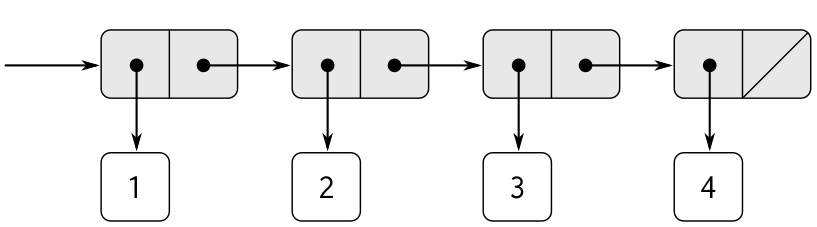
\includegraphics[width=0.5\textwidth]{figs/list}
        \end{center}
    \end{frame}

    \begin{frame}[fragile]{Моделируем список}
        \pause
        \begin{block}{API списков}
            \begin{itemize}
                \item $\term{nil}$ --- пустой список
                \item $\term{cons} \ap x \ap t$ --- список из элемента $x$ в голове и списка-хвоста $t$
                \item[\eg] $\tlist{\term{1}, \term{2}, \term{3}} \eqt \pause \term{cons} \ap \term{1} \ap (\term{cons} \ap \term{2} \ap (\term{cons} \ap \term{3} \ap \term{nil}))$
                \item Элиминатор, аккумулирующий элементы: $\term{fold}$
                \item[\eg] $\term{fold} \ap \tlist{\term{1}, \term{2}, \term{3}} \ap f \ap ini \eqbeta f \ap \term{1} \ap (f \ap \term{2} \ap (f \ap \term{3} \ap ini))$
            \end{itemize}
        \end{block}
        \pause
        \begin{block}{Законы списков}
            \begin{enumerate}
                \item \pause $\forall f~ini\ldotp \term{fold} \ap \term{nil} \ap f \ap ini \eqbeta \pause ini$
                \item \pause $\forall x~t~f~ini\ldotp \term{fold} \ap (\term{cons} \ap x \ap t) \ap f \ap ini \eqbeta \pause f \ap x \ap (\term{fold} \ap t \ap f \ap ini)$
            \end{enumerate}
        \end{block}
    \end{frame}

    \begin{frame}[fragile]{Списки в Си \popslide}
        \begin{minted}{C}
            struct Node {
                int value;
                Node * tail;
            };

            Node * nil = NULL;

            Node * cons(int value, Node * tail) {
                return new Node { value, tail };
            }
        \end{minted}
    \end{frame}

    \begin{frame}[fragile]{Списки на вариантах}
        \begin{block}{Законы списков}
            \begin{enumerate}
                \item \pause $\forall f~ini\ldotp \term{fold} \ap \term{nil} \ap f \ap ini \eqbeta \pause ini$
                \item \pause $\forall x~t~f~ini\ldotp \term{fold} \ap (\term{cons} \ap x \ap t) \ap f \ap ini \eqbeta \pause f \ap x \ap (\term{fold} \ap t \ap f \ap ini)$
            \end{enumerate}
        \end{block}
        \pause
        \begin{block}{Конструкторы}
            \begin{itemize}
                \item Вершина либо пустая, либо пара из элемента и хвоста
                \item $\term{nil} \termdef \pause \term{inl} \ap \term{0}\footnote{Произвольный терм, чтобы удовлетворить интерфейсу вариантов.}$
                \item $\term{cons} \ap x \ap t \termdef \pause \term{inr} \ap (\term{pair} \ap x \ap t)$
            \end{itemize}
        \end{block}
        \pause
        \begin{block}{Элиминатор}
            \[
                \begin{array}{l}
                    \term{fold} \ap xs \ap f \ap ini \termdef \pause \term{either} \ap \pause (\term{K} \ap ini) \ap \pause (\lambda (\term{pair} \ap x \ap t)\ldotp f \ap x \ap (\term{fold} \ap t \ap f \ap ini)) \ap \pause xs
                \end{array}
            \]
        \end{block}
    \end{frame}

    \begin{frame}[fragile]{Списки Чёрча (``наоборот'')}
        \begin{block}{Законы списков}
            \begin{enumerate}
                \item \pause $\forall f~ini\ldotp \term{fold} \ap \term{nil} \ap f \ap ini \eqbeta \pause ini$
                \item \pause $\forall x~t~f~ini\ldotp \term{fold} \ap (\term{cons} \ap x \ap t) \ap f \ap ini \eqbeta \pause f \ap x \ap (\term{fold} \ap t \ap f \ap ini)$
            \end{enumerate}
        \end{block}
        \pause
        \begin{block}{Конструкторы}
            \begin{itemize}
                \item По аналогии с числами Чёрча $\term{k} = \lambda s~z\ldotp \underbrace{s~(s~(\cdots (s~(}_{\textstyle k} z\underbrace{)\cdots ))}_{\textstyle k}$
                \item $\term{nil} \termdef \lambda s~z \ldotp z$
                \item $\term{cons} \ap x \ap t \termdef \pause \lambda s~z\ldotp \pause s~x~(t~s~z)$
            \end{itemize}
        \end{block}
        \pause
        \begin{block}{Элиминатор}
            \begin{itemize}
                \item $\term{fold} \ap xs \ap f \ap ini \termdef xs \ap f \ap ini$
                \item $\term{fold} \eqeta \term{id}$
            \end{itemize}
        \end{block}
    \end{frame}

    \begin{frame}[fragile]{Задачки про списки}
        \[\tlist{M_0, M_1, \cdots, M_{k-1}} \termdef \lambda s~z\ldotp \underbrace{s~M_0~(s~M_1~(\cdots (s~M_{k-1}~(}_{\textstyle k} z\underbrace{)\cdots ))}_{\textstyle k}\]
        \begin{itemize}
            \item[\todo] Напишите проверку на пустоту списка
            \item[\todo] Напишите конкатенацию списков
            \item[\todo] Напишите взятие головы списка
            \item[\answer] \pause
            \begin{columns}[onlytextwidth]
                \begin{column}{0.485\textwidth}
                    \[\term{isZero} \ap n \termdef n~(\lambda z'\ldotp \term{false})~\term{true}\]
                    \vspace{-1.5em}
                \end{column}\hfill\pause%
                \begin{column}{0.485\textwidth}
                    \[\term{isEmpty} \ap l \termdef \pause l~(\lambda x~z'\ldotp \term{false})~\term{true}\]
                    \vspace{-1.5em}
                \end{column}
            \end{columns}
            \item[\answer] \pause $\term{plus} \ap n \ap m \termdef \lambda s~z\ldotp n~s~(m~s~z)$
            \item[\answer] \pause
            \begin{columns}[onlytextwidth]
                \begin{column}{0.485\textwidth}
                    \[\begin{array}{l l}
                          \term{headOrDefault}~\textbf{nil}~d        & \eqt d \\
                          \term{headOrDefault}~(\textbf{cons}~x~t)~d & \eqt x
                    \end{array}\]
                    \vspace{-1.5em}
                \end{column}\hfill\pause%
                \begin{column}{0.485\textwidth}
                    \[\term{headOrDefault} \ap xs \termdef \pause xs \ap \mathbf{K}  \text{ или } \pause \textbf{fst}\]
                    \vspace{-1.5em}
                \end{column}
            \end{columns}
        \end{itemize}
    \end{frame}


    \sectionplan{Энергичность и ленивость}

    \begin{frame}[fragile]{Условное выражение как функция}
        Возьмём какой-нибудь привычный язык программирования.
        Эквивалентен ли код?
        \vspace{-1em}
        \begin{columns}[onlytextwidth]
            \begin{column}[t]{0.485\textwidth}
                \begin{minted}{python}

                    if b:
                        return f()
                    else:
                        return g()
                \end{minted}
            \end{column}\hfill%
            \begin{column}[t]{0.485\textwidth}
                \begin{minted}{python}
                    def myif(cond, t, e):
                        if cond:
                            return t
                        else:
                            return e
                    myif(b, f(), g())
                \end{minted}
            \end{column}
        \end{columns}
        \pause
        Нет, например:
        \vspace{-1em}
        \begin{columns}[onlytextwidth]
            \begin{column}[t]{0.485\textwidth}
                \begin{minted}{python}
                    def fac(n):
                        if n <= 1:
                            return 1
                        else:
                            return n * fac(n - 1)
                \end{minted}
            \end{column}\hfill%
            \begin{column}[t]{0.485\textwidth}
                \begin{minted}{python}
                    def fac(n):
                        return myif(n <= 1,
                            1,
                            n * fac(n - 1)
                        )
                \end{minted}
            \end{column}
        \end{columns}
        \vspace{1em}
        Что произойдёт? \pause Вычисление разойдётся.
        \begin{minted}{python}
            fac(3) -> myif(n <= 1, 1, n * fac(n - 1)) #\pause#
                   -> myif(n <= 1, 1, n * myif(n - 1 <= 1, 1, (n - 1) * fac(n - 1 - 1))...
        \end{minted}
    \end{frame}

    \begin{frame}[fragile]{Энергичная и ленивая семантики вычисления}
        \pause
        \vspace{-0.7em}
        \begin{block}{Подстановочная модель вызова}
            Вызов функции означает подстановку текста её тела в место вызова.
        \end{block}
        \pause
        \vspace{-0.3em}
        \begin{block}{Энергичная семантика вычислений}
            Аргументы функции вычисляются до её вызова (подстановки).
        \end{block}
        \pause
        \vspace{-0.3em}
        \begin{block}{Ленивая семантика вычислений}
            Сначала происходит вызов функции, аргументы без необходимости не вычисляются.
        \end{block}
        \pause
        От энергичной семантики можно перейти к ленивой, как? \pause Лямбды!
        \pause
        \vspace{-1em}
        \begin{columns}[onlytextwidth]
            \begin{column}[t]{0.485\textwidth}
                \begin{minted}{python}
                    def fac(n):
                        return myif(n <= 1,
                            lambda: 1,
                            lambda: n * fac(n - 1)
                        )
                \end{minted}
            \end{column}\hfill%
            \begin{column}[t]{0.485\textwidth}
                \begin{minted}{python}
                    def myif(cond, t, e):
                        if cond:
                            return t()
                        else:
                            return e()
                \end{minted}
            \end{column}
        \end{columns}
    \end{frame}


    \sectionplan{Материалы}

    \begin{frame}{Что посмотреть в транспорте}
        \begin{itemize}
            \item \href{https://habr.com/ru/articles/486548/}{\color{blue} Статья: Примитивно-рекурсивные функции и функция Аккермана}
        \end{itemize}
    \end{frame}

    \begin{frame}{Серьёзные материалы}
        \begin{itemize}
            \item \href{http://www.cs.ru.nl/barendregt60/essays/klop/art16_klop.pdf}{\color{blue} Klop, J. W. ``New fixed point combinators from old.'' Reflections on Type Theory, $\lambda$-Calculus, and the Mind. Essays dedicated to Henk Barendregt on the occasion of his 60th birthday, Radboud University Nijmegen (2007): 197--211.197--211}
        \end{itemize}
    \end{frame}

\end{document}
